%---------------------------------------------------------------------
%
%                          Cap?tulo 4
%
%---------------------------------------------------------------------

\chapter{Materiales}


\label{cap4:sec:kinect}
En este cap�tulo se expondr�n los  materiales  y m�todos utilizados para el desarrollo del proyecto. A continuaci�n se detallar�n de forma t�cnica las tecnolog�as y los dispositivos utilizados para realizar el proyecto.


%-------------------------------------------------------------------
\section{Software y hardware empleados}
%-------------------------------------------------------------------
\label{cap4:sec:Software y hardware empleados}
El software principal utilizado en este proyecto es Unity 5.5 (poner referencia), que es un motor de desarrollo de videojuegos.
Para la edici?n , compilaci?n y depuraci?n de la programaci?n de Unity se ha utilizado Visual Studio 2015 (poner referencia) con el lenguaje de programaci?n C\#.\\
\\
\comImpl{Aqui raul pones los programas de modelado de avatar. Animaciones de mixamo,.}\\
\\

El hardware principal usado en este proyecto es el dispositivo de captura de movimiento kinect v2 (referencia) y el cable de conexion(nose como se llama, referencia).







\subsection{Entorno de desarrollo : Unity 3D}
%-------------------------------------------------------------------
\label{cap4:sec:Entorno de desarrollo : Unity 3D}
El objetivo de este proyecto es la captura y el an?lisis de movimiento relacionados con el arte marcial afro-brasile?o capoeira(?referencia?). Con esto en mente, se llega a la primera decisi?n de que plataforma escoger para el desarrollo de este proyecto.\\

Los entornos a elegir ser?an Visual Studio 2015, Unity 3D y Unreal Engine 4 (referencia). El primero descartado es desarrollar directamente en Visual Studio 2015 porque se busca crear tambi?n un escenario 3D y, tanto Unity como Unreal ,facilitan la creaci?n de estos escenarios.\\\\
En cuanto a la decisi?n de elegir entre Unity 3D o Unreal Engine 4 fue basada en la comunidad que hay detr?s de cada uno de ellos, y sobre todo, en lo que se quiere abarcar con este proyecto. Unreal suele ser utilizado por las empresas para juegos grandes y mas profesionales , mientras que Unity se puede aplicar a peque?as y grandes aplicaciones siendo su aprendizaje de este mas intuitivo que Unreal.
\\\\
Y por ultimo la elecci?n de lenguaje de programacion siendo el lenguaje de C\# una opci?n m?s sencilla para el desarrollo de este proyecto.(buscar diefrencias claras)


\section*{Comunidad de Unity}
 Video: 640x480 @30 fps
%-------------------------------------------------------------------
\subsection{Kinect V2}
%-------------------------------------------------------------------




\comImpl{Enlaces sobre las caracteristicas de Kinect}

\medskip
https://msdn.microsoft.com/library/jj131033.aspx\\
https://msdn.microsoft.com/library/dn782025.aspx\\
https://developer.microsoft.com/es-es/windows/kinect/hardware


\subsection{MakeHuman}

La aplicaci�n MakeHuman sirve para crear modelos humanos que pueden ser utilizados en diferentes plataformas 3D, como animaciones, videojuegos, etc. Promueve el arte digital y artistas digitales, proporcionando una herramienta de alta calidad liberada al dominio p�blico con la licencia CCO, mientras que la base de datos y el c�digo se publicaron mediante una licencia AGPL3.

\begin{figure}[h!]
	\centering
	
\includegraphics[width=0.8\linewidth, height=0.3\textheight]{Imagenes/Capitulos/4/logo_makehuman}
	\caption{Logo MakeHuman}
	\label{fig:logo_makehuman}
\end{figure}


MakeHuman utiliza un humano est�ndar y mediante varios deslizadores o scrolls se podr�n alterar los par�metros de la estatura, anchura, sexo, edad, etc. 


\begin{figure}[h!]
	\centering
	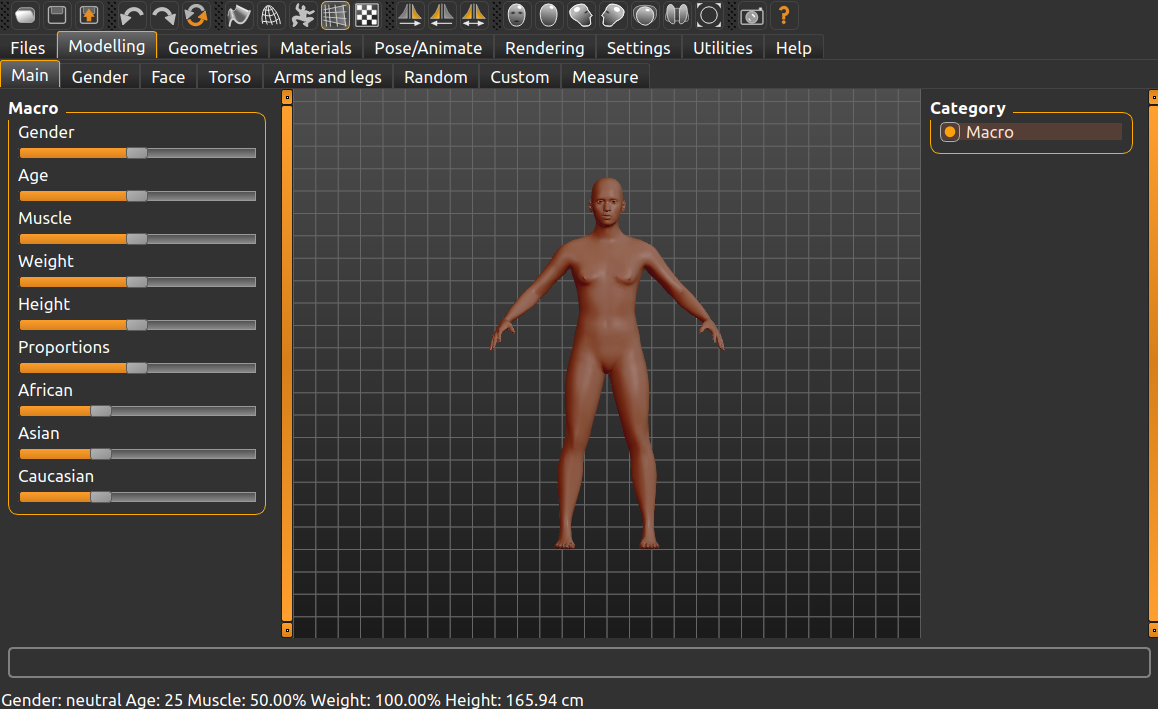
\includegraphics[width=0.8\linewidth, height=0.3\textheight]{Imagenes/Capitulos/4/makehuman_estandar}
	\caption{Aspecto del humano est�ndar de MakeHuman}
	\label{fig:makehuman_estandar}
\end{figure}

En un principio se pens� utilizar esta aplicaci�n para el modelado de los personajes debido a su intuitiva interfaz y la facilidad de exportaci�n en formato fbx el cual utiliza Unity. Pero tras investigar posibles alternativas, se encontr� la aplicaci�n Fuse Character Creator, la cual posibilitaba el desarrollo de los personajes con mayor calidad. De forma simultanea se podr�a realizar la configuraci�n de los personajes para su posterior animaci�n.

\subsection{Fuse Character Creator}

Se trata de una aplicaci�n desarrollada por Mixamo, la cual permite crear personajes �nicos mediante una intuitiva interfaz que separa el avatar en diferentes partes, como son la cabeza, el torso, las piernas y los brazos. Posteriormente a la selecci�n de las diferentes partes del cuerpo ya predefinidas por el sistema, se puede editar cada una de las partes del personaje, ya sean los rasgos de la cara, el tama�o de los brazos, la longitud de las piernas, etc. Al seleccionar la parte del cuerpo que se quiere modificar, simplemente ser� necesario pinchar y realizar un scrool o deslizamiento hacia la izquierda o derecha para aumentar su tama�o, y para seleccionar el punto exacto donde se ubicar� por ejemplo el ombligo, los ojos, las rodillas, etc, se realizar� un scrool o desplazamiento hac�a arriba o abajo.

Al terminar de modelar el personaje, se pasar� a la secci�n de vestuario. Donde existen prendas predefinidas, como camisas, pantalones, zapatos, etc. Al terminar de vestir al avatar, esta aplicaci�n posee la peculiaridad de poder subir al servidor de Mixamo el modelado realizado y completar la configuraci�n de los huesos adem�s de incluir una posible animaci�n.


\subsection{Mixamo}

\subsection{Marvelous Designer}
\subsection{Blender}


%Y tambi?n ponemos el acr?nimo \ac{CVS} para que no cruja.

%Ten en cuenta que si no quieres acr?nimos (o no quieres que te falle la compilaci?n en ``release'' mientras no tengas ninguno) basta con que no definas la constante \verb+\acronimosEnRelease+ (en \texttt{config.tex}).


%-------------------------------------------------------------------
%\section*{\ProximoCapitulo}
%-------------------------------------------------------------------



% Variable local para emacs, para  que encuentre el fichero maestro de
% compilaci?n y funcionen mejor algunas teclas r?pidas de AucTeX
%%%
%%% Local Variables:
%%% mode: latex
%%% TeX-master: "../Tesis.tex"
%%% End:
